\documentclass{beamer}
\usepackage{hyperref}
\usepackage{xcolor}
\usepackage{graphicx}

\newcommand{\credit}[1]{\par\hfill \footnotesize Fonte:~\itshape#1}
\newcommand{\link}[2]{\color{blue}{\underline{\href{#1}{#2}}}}

\graphicspath{{./img/}}

\usetheme{AnnArbor}
\usecolortheme{orchid}
\title{ERP: L'area logistica}
\author{Blascovich Alessio, Fontanive Piero}
\date{}

\begin{document}
\begin{frame}
    \titlepage
\end{frame}

\section{Obbiettivi}
\begin{frame}{Obbiettivi}
    La parte di sistema informativo rivolto alla logistica si occupa di:
    \begin{itemize}
        \item Tenere traccia del movimento della merce.\\
            \textit{Fornisce anche API per tracciare il pacco dall'esterno come i vari corrieri espresso.}
        \item Fornire dati analitici sulla merca.\\
            \textit{E' possibile fare un resoconto sulla disponibilità è la giacenza degli articoli.}
        \item Effettuare previsioni sullo stato dell'inventario.\\
            \textit{Dopo il black friday avrò bisogno di ordinare x unità di articolo 1 e y unità di articolo 2.}
    \end{itemize}
\end{frame}

\subsection{Evoluzione obbiettivi}
\begin{frame}{Evoluzione obbiettivi}
    Nei sistemi più grandi ed evoluti è possibile compiere funzioni per:
    \begin{itemize}
        \item Localizzare a livello fisico l'ubicazione di un articolo.
        \item Tracciare origine e destinazione di un lotto di articoli o di un singola tipologia di articoli usandone la marticola.
        \item Muovere parzialmente o totalmente la merce in automatico.\\
            ome viene fatto nei magazzini di alcune multinazionali, un esempio può essere \link{https://www.youtube.com/watch?v=YL9XjyXsKKk}{questo}.
    \end{itemize}
\end{frame}

\section{Strutture di base}
\begin{frame}{Strutture di base}
    La logistica si avvale di tre strutture base:
    \begin{enumerate}
        \item L'anagrafica degli articoli, ovvero la descrizione dei prodotti che un'azienda gestisce.
        \item La compisizione fisica e logica del magazzino dove si andrà ad operare.
        \item La movimentazione degli articoli, ovvero la rappresentazione dei movimenti compiuti.
    \end{enumerate}
\end{frame}

\subsection{Nominazione articoli}
\begin{frame}{Nominazione articoli -  Intro}
    Un problema fondamentale è la standardizzazione nella nomenclatura della merce all'interno di un azienda.\\
    E' necessario trovare metodi di nomenclatura che creaino meno \textbf{omocodia} possibile e che siano facilmente leggibili.\\
    \vspace{1.5em}
    \textbf{E.g.}\\
    Una numerazione progressiva è facile da implementare ma crea difficoltà nella correlazione numero -$>$ prodotto.\\
    Il codice fiscale crea omocodie, nel 2015 erano presenti 35800 casi di persone vive con codici uguali.
    \credit{\link{https://www.agenziaentrate.gov.it/portale/documents/20143/318757/Audizione+del+Direttore+dell+Agenzia+delle+Entrate+10+02+2016_Audizione+-+Codice+Fiscale+e+Omocodie+-+10+feb+2016+df.pdf/202e5395-f622-62e5-219a-7ce894d538a4}{Agenzia delle entrate}}
\end{frame}

\begin{frame}{Nominazione articoli - Piano di codifica}
    Per evitare i problemi visti prima si ricorre ad un \textbf{piano di codifica}, ovvero il processo che permette di definire un nome univoco.\\
    Per la definizione del nome si usano prevalentemente due sistemi a codifica:
    \begin{enumerate}
        \item lineare
        \item condizionata
    \end{enumerate}
\end{frame}

\subsection{Codifiche lineari e condizionali}
\begin{frame}{Nominazione articoli - Codifiche lineari e condizionali}
    \begin{enumerate}
        \item \textbf{Codifica lineare:} viene scelto un insieme di caratteri che identifichi ogni articolo tramite una stringa, tipicamente lunga dai 15 ai 20 caratteri.\\
            Le stringhe vengono generate facendo un intersezione tra tutte le caratteristiche scelte, ogni intersezione tra tutte le caratteristiche deve avere al ppiù un elemento.
        \item \textbf{Codifica condizionale:} non viene usata una semplice concatenazione di lunghezza fissa ma di scegliere ad ogni passaggio la parte del codice in base al codice già scelto nelle fasi precedenti.
    \end{enumerate}
\end{frame}

\subsection{Esempio}
\begin{frame}{Nominazione articoli - Esempio}
    Un'azienda prodice sedie e tavoli, (MO) modello sedia, (AS) altezza sedia, (AC) altezza schienale, (MF) materiale del fusto, (MT) modello tavolo, (DP) dimensione del piano, (MP) materiale del piano, (MG) materiale delle gambe \dots\\
    Infine un atributo (TP) che assume i valori S per le sedie e T per i tavoli.\\
    \begin{itemize}
        \item \textbf{Sedia:} TP+MO+AS+AC+MF+\dots
        \item \textbf{Tavolo:} TP+MT+DP+MP+MG+\dots
    \end{itemize}
    Questo però porta (nei casi più complessi) ad avere codici molto lunghi ma molto simili tra di loro, è bene quindi creare degli alias.\\
    \textbf{E.g.}\\
    \begin{itemize}
        \item \color{red}{Luxury01}
        \item \color{blue}{Luxury02}
    \end{itemize}
\end{frame}

\subsection{Codifiche parlanti e strutturate}
\begin{frame}{Nominazione articoli - Codifiche parlanti e strutturate}
    L'ultima decisione da prendere è scegliere la codifica nella quale verranno prodotti i codici di identificazine.\\
    Si presentano quindi, due scelte:
    \begin{enumerate}
        \item \textbf{Parlante:} questo tipo di codifica rende possibile all'utente di capire le caratteristiche dell'oggetto guardando solo il codice.
        \item \textbf{Strutturata:} questa codifica rende il codice più compatto, ma meno leggibile dall'utente.
    \end{enumerate}
    \textbf{E.g.}\\
    Facendo riferimento alla voce (MF) del materiale del fusto di una sedia.
    \begin{center}
        \begin{tabular}{|c|c|c|c|}
            \hline
            \textbf{Materiale} & \textbf{Codice parlante} & \textbf{Codice strutturato} \\
            \hline
            Ciliegio           & CIL                      & 0                           \\
            \hline
            Fagio              & FAG                      & 1                           \\
            \hline
        \end{tabular}
    \end{center}
\end{frame}

\subsection{Anagrafiche dei prodotti}
\begin{frame}{Anagrafiche dei prodotti}
    I sistemi informativi ragruppano in queste "anagrafiche" le principali informazioni necessarie al trattamento del articolo.\\
    Queste informazioni sono:
    \begin{itemize}
        \item Il codice dell'articolo, che identifica univocamente l'oggetto.
        \item Descrizione articolo, che in alcuni sistemi è formata in modo automatico partendo dal codice strutturato.
        \item Unità di misura, per quanto strano possa sembrare non è inusuale che un prodotto venga fabbricato in un unità di misura (kilogrammi) e venduto in un'altra (unità).
        \item Imballaggio e confezione.
    \end{itemize}
\end{frame}

\begin{frame}{Anagrafiche dei prodotti}
    \begin{itemize}
        \item Approvigionamento ovvero se un articolo viene acquistato oppure prodotto internamente.
        \item Politica di gestione, le più comuni forme sono \textit{a scorta} e \textit{a fabisogno}.
        \item Movimentazione che indica se l'articolo è fisico oppure se è presente per pure informazioni di anagrafica.
        \item Stato:
            \begin{itemize}
                \item In esaurimento.
                \item Esaurito.
            \end{itemize}
        \item Scheda tecnica, è possibile associare ad un articolo dei file descrittivi come immagini, progetti CAD \dots
    \end{itemize}
\end{frame}

\subsection{Informazioni di approvigionamento e produttive}
\begin{frame}{Anagrafiche dei prodotti - Informazioni di approvigionamento e produttive}
    Gli ERP contengono anche informazioni per quanto riguarda gli acquisi, la varietà di queste informazioni varia da contesto a contesto ma generalmente sono sempre presenti:
    \begin{itemize}
        \item Lead time, il tempo che impiega la merce ad arrivare.
        \item Scorta minima che rappresenta la quantità che serve a far fronte a picchi di ordini.
        \item Livello di riordino ovvero la quantità che serve a far fronte ad un lungo periodo come il lead time.
    \end{itemize}
\end{frame}

\begin{frame}{Anagrafiche dei prodotti - Informazioni di approvigionamento e produttive}
    \begin{center}
        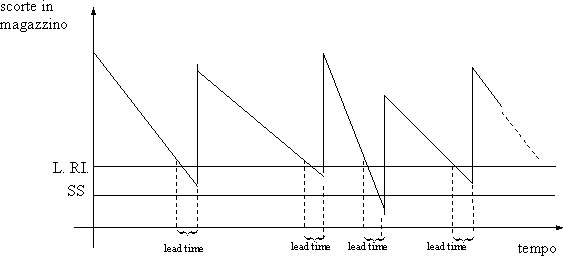
\includegraphics[scale=0.5]{livello_di_riordino.png}
    \end{center}
\end{frame}

\subsection{Informazioni da contenere}
\begin{frame}{Anagrafiche dei prodotti - Informazioni da contenere}
    Ogni articolo deve contenere alcune informazioni di base come:
    \begin{itemize}
        \item Info sul fornitore dell'articolo.
        \begin{itemize}
            \item Nome fornitore.
            \item Lead time.
            \item Lotto minimo ordinabile.
        \end{itemize}
        \item Informazioni sui clienti che vanno ad acquistare l'articolo.
        \begin{itemize}
            \item Nome cliente.
            \item Descrizione personalizzata dal cliente.
            \item Imballaggio personalizzato.
            \item Etichettature specifiche.
        \end{itemize}
        \item I dati economici sull'articolo.
        \begin{itemize}
            \item Aliquota IVA.
        \end{itemize}
    \end{itemize}
\end{frame}

\subsection{Layout aziendale}
\begin{frame}{Layout aziendale}
    Solitamente il layout di un'azienda arriva ad essere molto complesso e vasto, diamo quindi due definizioni:
    \begin{itemize}
        \item \textbf{Deposito:} l'ubicazione fisica in cui sono presenti gli articoli.
        \item \textbf{Magazzino:} l'insieme di tutti i deposizi di un'azienda.
    \end{itemize}
\end{frame}

\section{Flussi evoluti}
\begin{frame}{Flussi evoluti}
    I sistemi informativi evoluti offrono molte altre funzioni per un trattamento adeguato della logistica.\\
    Spesso, quando la complessità è elevata o i processi sono molto verticali, l'ERP lascia il posto a sottosistemi di logistica mirati, che interfacciano la strumentazione di campo (quali, per esempio, lettori di codici a barre) per facilitare il tracciamento delle operazioni. Nel seguito descriveremo sommariamente i seguenti temi, gestiti dai principali sistemi ERP:\\
    \begin{itemize}
        \item \textbf{Lotti}
        \item \textbf{Matricole}
        \item \textbf{Ubicazioni/celle}
    \end{itemize}
\end{frame}

\subsection{Magazzino a Lotti}
\begin{frame}{Magazzino a Lotti}
    Quando la logistica è gestita in parte o interamente a lotti, si desidera tracciare un insieme di informazioni comuni proprie di un particolare gruppo di oggetti “articolo”, che si differenziano da quelle di un altro gruppo del medesimo articolo.\\
    \vspace{1.5em}
    \textbf{E.g.}\\
    Si consideri, per esempio, il processo produttivo di un medicinale. In una determinata giornata le confezioni di medicinale prodotte sono associate a un particolare lotto di produzione, che ha una sua data di scadenza; il giorno successivo si ha un altro lotto dello stesso medicinale, con un'altra data di scadenza.
\end{frame}

\begin{frame}{Magazzino a Lotti - Strutture di riferimento}
    \begin{itemize}
        \item Informazioni di nominazione/identificazione;
        \begin{itemize}
            \item \textbf{E.g.} 2018-VER-00023
        \end{itemize}
        \item Informazioni logistiche;
        \begin{itemize}
            \item \textbf{E.g.} giacenza, ubicazione
        \end{itemize}
        \item Informazioni di stato;
        \begin{itemize}
            \item Accettato/da analizzare/scaduto/respinto/sospeso/difettoso.
        \end{itemize}
    \end{itemize}
\end{frame}

\begin{frame}{Magazzino a Lotti - Strutture di riferimento}
    \begin{itemize}
    \item Informazioni di tracciabilità;
        \begin{itemize}
            \item Dalla sorgente:
            \begin{itemize}
                \item fornitura esterna;
                \item denuncia di produzione;
                \item carico per movimentazione interna.
            \end{itemize}
            \item Dalla terminazione:
            \begin{itemize}
                \item vendita;
                \item prelievo per produzione;
                \item prelievo per movimentazione interna.
            \end{itemize}
        \end{itemize}
        \item Informazioni fisico/dimensionali/gestionali.
        \begin{itemize}
            \item data produzione del fornitore;
            \item data scadenza;
            \item umidità;
            \item peso;
            \item volume;
            \item numero serie iniziale e finale;
            \item qualità.
        \end{itemize}
    \end{itemize}
\end{frame}

\begin{frame}{Magazzino a Lotti - Procedure di alimentazione}
    Le procedure di alimentazione prevedono che in tutti i punti in cui c'è una movimentazione di magazzino vengano o richiesti o calcolati automaticamente i lotti di riferimento.
    \begin{itemize}
        \item \textbf{Ricezione materiali}: creazione dei lotti (punto sorgente);
        \item \textbf{Spedizione materiali}: chiusura totale o parziale dei lotti (punto terminazione);
        \item \textbf{Controllo qualità}: movimentazione dei lotti;
        \item \textbf{Movimentazione produttiva}: chiusura totale o parziale dei lotti utilizzati (punto terminazione) e creazione dei nuovi lotti (punto sorgente);
        \item \textbf{Movimentazione logistica interna}: movimentazione dei lotti.
    \end{itemize}
\end{frame}

\begin{frame}{Magazzino a Lotti - Procedure di analisi e controllo}
    Solitamente le operatività gestionali si limitano ad analisi della situazione per lotto. Le più comuni sono:
    \begin{itemize}
        \item giacenze/impegni di articoli divisi per lotto ed eventualmente per ubicazione;
        \item lotti in scadenza;
        \item lotti nei vari stati;
        \item lotti che soddisfano particolari caratteristiche:
        \begin{itemize}
            \item \textbf{E.g.} con una percentuale di umidità maggiore del 70\%.
        \end{itemize}
    \end{itemize}
    Oltre a queste vi sono tutte le funzioni che permettono il tracciamento dei lotti. Nei sistemi più evoluti il tracciamento è rappresentato graficamente, con possibilità di navigazione dai singoli nodi verso i documenti associati.
\end{frame}

\subsection{Magazzino a Matricole}
\begin{frame}{Magazzino a Matricole}
    \begin{itemize}
        \item Numeri di serie;
        \item Numeri di matricole;
    \end{itemize}
\end{frame}

\end{document}